
\documentclass[preprint,12pt]{elsarticle}

\usepackage[spanish]{babel}
\usepackage{amssymb}
\usepackage{graphicx}
\usepackage{lineno}
\usepackage[utf8]{inputenc}
\usepackage{url}
\usepackage{color}
\usepackage[hidelinks]{hyperref}


\begin{document}
	
	\begin{frontmatter}
		
		
		\title{\huge Data Storytelling}
		
		\author{Mamani Ayala, Brandon        (2015052715)}
		\author{Quispe Mamani, Angelo	      (2015052826)}
		\author{Vizcarra Llanque, Jhordy	      (2015052719)}
		\author{Ordoñez Quilli, Ronald          (2015052821)}
		\author{Rodriguez Mamani, Juan      (2017057862)}
		
		\address{Tacna, Perú}
		
		\begin{abstract}
			%% Text of abstract
			Data StoryTelling (narración de datos) está ganando rápidamente protagonismo como una actividad característica del periodismo digital con una adopción significativa por parte de pequeñas y grandes empresas de medios. Si bien un puñado de estudios anteriores han examinado qué caracteriza aspectos de la narración de datos, como narraciones y visualización o análisis basados en casos individuales, todavía no hemos visto un esfuerzo sistemático para aprovechar estos recursos disponibles para obtener una mejor comprensión de lo que caracteriza a las buenas historias de datos y cómo estos son creados.Este articulo presenta informacion sobre Data Storytelling que para el conocimiento. 


	
		\end{abstract}
\end{frontmatter}
%%

	
	%%
	%\linenumbers
	
	%% main text
	\section{Resumen}

El Data Storytelling es esencial en una empresa. Esto porque se trata de una manera de dar sentido a los datos, junto a una nueva o mejor perspectiva y, además, mejorando su interpretación. Esto ayuda a simplificar y hacer que los datos sean más relevantes, significativos e interesantes.

De la misma manera, es la forma más práctica para dar a conocer y entender la importancia de los datos.

Además, ten en cuenta que las historias que tienen datos y análisis son siempre las más convincentes. Esto se debe a que combinan datos que involucran personas y organizaciones, una mezcla que genera más confianza en el público.

Data Storytelling para Empresas hoy en día narrar una historia con datos es un factor clave en la toma de decisiones. También es una forma rápida de hacer digerible y comprensible la información que deseas transmitir. Es la mejor vía para que tu empresa pueda identificar los problemas y actuar rápidamente.

Ten presente que la Data Storytelling no se trata sólo de narrar algo que deseas vender, sino que cuenta lo que muestran los datos. Es un trabajo donde lo fundamental es hacer razonable la información recabada, procesarla, resaltar su valor, visualizarla y transmitirla.
	El Data StoryTelling posee tres componentes esenciales para poder cumplir con su función de forma óptima. Con ellos logra entregar la información necesaria de forma clara, convincente y transmitiendo mucho más que solo datos. 
		\begin{itemize}
		\item  Historia: Es donde se construye el relato a partir de los pitch (Esquema narrativo y el desarrollo), elementos principales de la historia.
		\item Soporte Virtual: Donde se incluyen gráficas dinámicas e interactivas, con colores llamativos y bien escogidos y tamaños de fuente adecuados. El soporte visual debe contener mensajes muy claros que permitan comprender qué es lo realmente importante.
		\item El Presentador: Es quien narra la historia que se transmite. Este debe ser excelente para narrar, ya que, si tienes un buen escenario, un excelente soporte visual, pero un pésimo presentador, entonces el mensaje no llegará de forma exitosa.
	\end{itemize}

	%%
	
	%%
	%\linenumbers
	
	%% main text

\section{Objetivos}
		\begin{itemize}
		\item Objetivo 1: En primer lugar, la importancia radica en la riqueza de la información con la que se cuenta dentro de una base de datos y el aporte que ésta brinda al momento de contar una historia.
		\item Objetivo 2: Permite simplificar toda la información que las organizaciones quieren transmitir a sus diferentes grupos de interés, ya sean clientes, colaboradores, proveedores, accionistas.
		\item Objetivo 3: Permite representar de manera más sencilla y dinámica el mensaje. Empleando la narrativa, logramos que el mensaje sea interpretado de la manera en que deseamos.
	\end{itemize}

	%%
	
	%%
	%\linenumbers
	
	%% main text

\section{Marco Teorico}
	
\subsection{Elementos clave}	
	El llamado Data Storytelling no es más que un enfoque estructurado sobre cómo comunicamos insights a partir de los datos, e involucra una combinación de 	tres elementos: datos, visualización y narrativa.
	\begin{center}
	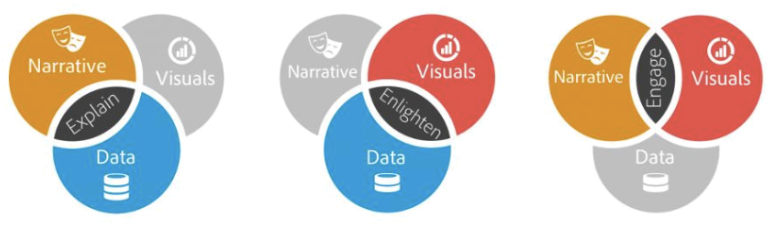
\includegraphics[width=15cm]{./Imagenes/imagen1} 
	\end{center}
\begin{itemize}
\item	Narrativa + Datos = podremos explicar qué ha pasado y por qué un insight puede ser importante. Necesitaremos contexto para entender las conclusiones por completo.
\item Visualización + Datos = Enlighten. Cuando añadimos una visualización a nuestros datos, podemos iluminar a nuestra audiencia con insights que no habrían visto de otra manera.
\item	Narrativa + Visualización = Engagement. La combinación perfecta para lograr ese interés e incluso para entretener a nuestra audiencia. 
\end{itemize} 

	Pero, cuando unimos Visualización + Narración + Datos = Change, logramos contar una historia con nuestros datos, logramos influenciar y llevar a ese 			cambio que estábamos buscando.

	\begin{center}
	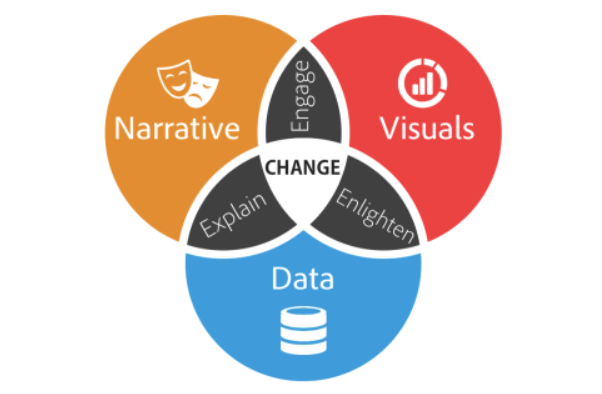
\includegraphics[width=10cm]{./Imagenes/imagen2} 
	\end{center}
Y es que la pasión por los datos, ¡tiene que ir acompañada también por la pasión de contar historias! Si comunicas pobremente tus insights o si llegas a conclusiones erróneas, puede ser prácticamente peor que no utilizar ningún dato.

\subsection{¿Por qué Data Storytelling?}
Si no tienes claro por qué incluir el elemento “historia” en tus análisis o no estás seguro de que vaya a funcionar, estos cuatro puntos te ayudarán a cambiar de opinión:

\begin{itemize}
\item	1.	Las historias son herramientas efectivas para transmitir la experiencia humana: esto ha sido así desde el inicio de los tiempos, pero ahora utilizamos datos y análisis para crear versiones mejoradas de esas historias. Gracias a ellas simplificamos y damos sentido a un mundo complejo.
\item 2.	Para inspirar el cambio, necesitamos que entiendan nuestra historia: no importa cuántas horas hay detrás de nuestro análisis, no lograremos nada si no nos logramos explicar ya sea con una narrativa o con gráficos pero, necesitamos una historia.
\item 3.	Las personas quieren evidencia del análisis que hay detrás: aunque nuestra audiencia no entienda el detalle de la analítica, sí quieren la evidencia de que hay datos detrás, ya que estas historias son más convincentes que solo una experiencia personal.
\item	4.	Contar en una breve historia el resultado de horas de trabajo: se necesitan presentaciones cortas, con ideas concretas adaptadas a los stakeholders que recibirán la información para hacer llegar tu mensaje de una manera simple. \\
	\begin{center}
	
\includegraphics[width=10cm]{./Imagenes/imagen3} 
	\end{center}
\end{itemize} 


\subsection{Data Visualization}
	Es muy común que Data Storytelling se entienda solo como visualización de datos y, aunque como estamos viendo, es mucho más que eso, es cierto que la visualización es una parte esencial y muy potente como complementaria al análisis, para poder condensar grandes conjuntos de datos en una sola foto.

\subsection{Pero, ¿qué nos permite?}
	
\begin{itemize}
\item	1.	Comprensión rápida de la información: gracias a las representaciones gráficas podemos ver grandes cantidades de datos de forma clara y coherente, lo que facilita la extracción de conclusiones e insights. Ganaremos tiempo y eficiencia para solucionar problemas.
\item 2.	Identificar y actuar rápido sobre tendencias emergentes: incluso los archivos de datos casi infinitos, empiezan a tener sentido al representarse gráficamente; lo que nos permite detectar parámetros que están altamente correlacionados. Algunas relaciones serán obvias, pero otras tendremos que identificarlas para ayudar al cliente a enfocarse en ese punto de mejora que influenciará en sus objetivos principales.
\item 3.	Identificar relaciones y patrones dentro de los activos digitales: descubrir tendencias dentro de los datos nos puede dar ventaja competitiva, como detectar puntos clave que están afectando a la calidad del producto o solucionar incidencias antes de que se conviertan en mayores problemas.
\item	 4.	Desarrollar un nuevo lenguaje de negocio para contar la historia a otros: una vez que hemos descubierto nuevos insights gracias a la analítica visual, el siguiente paso es comunicarlos, ya sea con gráficos simples o visualizaciones elaboradas, pero lo importante es lograr ese engagement y transmitir el mensaje rápidamente. \\

	\begin{center}
	
\includegraphics[width=10cm]{./Imagenes/imagen4} 
	\end{center}
\end{itemize} 

	%%

	%%
	%\linenumbers
	
	%% main text

\pagebreak
\section{Ejemplo}
	
\subsection{Contar una historia convincente}	
Este ejemplo destaca claramente a una compañía con múltiples ubicaciones de negocios en la forma en que sus objetivos se superponen en sus diferentes ubicaciones. Esto es importante para el propietario del negocio, ya que la orientación de ubicaciones que se superponen en las campañas de búsqueda puede provocar la canibalización de los datos y la libre competencia. 
\begin{center}
	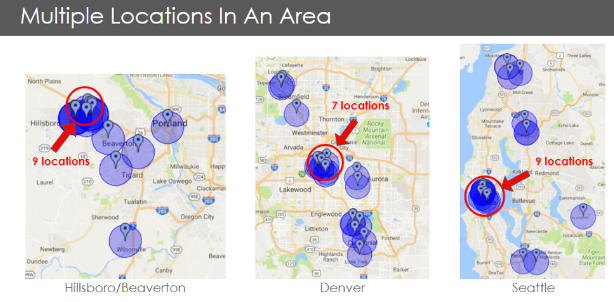
\includegraphics[width=10cm]{./Imagenes/ejemplo1} 
\end{center}

\subsection{Proporcionar contexto}	
Este tipo de información para un informe del cliente podría haberse distribuido fácilmente en una lista de viñetas, pero en su lugar, se presenta como una línea de tiempo clara y nítida. Nuestra agencia envía a los clientes informes mensuales y puede ser fácil olvidarse de los cambios grandes e impactantes que se hicieron en una cuenta cuando se presentan en medio de muchas otras mediciones, tendencias, pequeños ajustes, etc. 
\begin{center}
	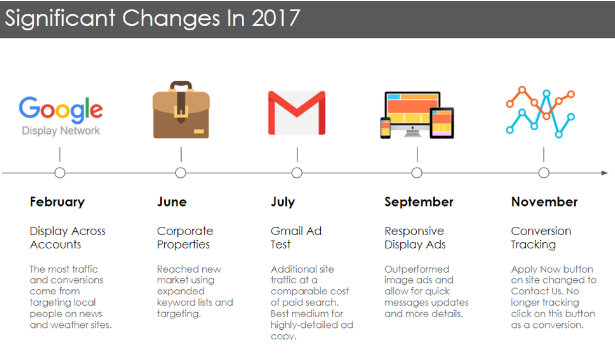
\includegraphics[width=10cm]{./Imagenes/ejemplo2} 
\end{center}

\subsection{Terminar con una perspicacia}	
Este ejemplo en particular fue parte de una presentación que ilustra la importancia del seguimiento de las visitas a la tienda. Muchos de nuestros clientes, y muchos dueños de negocios en general, luchan por fusionar datos en línea y fuera de línea para crear una imagen completa de sus consumidores. Ser capaz de explorar cómo los usuarios descubren la marca, cómo se mantienen comprometidos y qué les lleva a actuar finalmente puede ser una información invaluable.
\begin{center}
	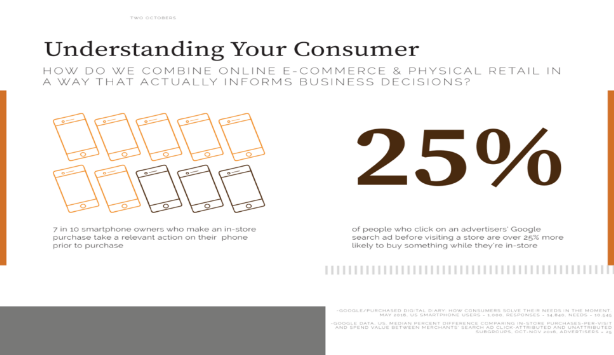
\includegraphics[width=10cm]{./Imagenes/ejemplo3} 
\end{center}

\subsection{Explique Con Visuales, Narrar Con Palabras}	
Esta diapositiva hace un trabajo maravilloso que ilustra el rendimiento de diferentes geo-objetivos dentro de una cuenta de búsqueda pagada. Es visualmente atractivo, y atrae a los usuarios con banderas que representan a cada país y medallas como indicadores de éxito. 
\begin{center}
	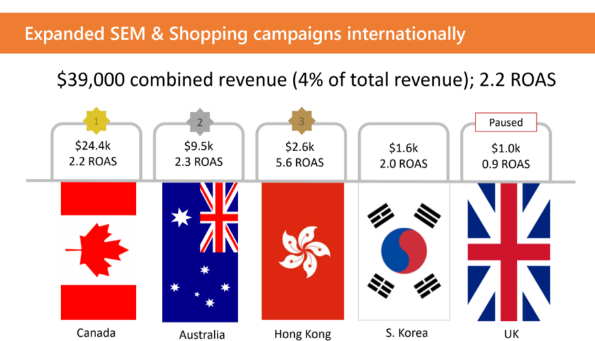
\includegraphics[width=10cm]{./Imagenes/ejemplo4} 
\end{center}



\pagebreak
\section{Analisis}
	

aqui el analisis

\newpage

%%
	
	%%
	%\linenumbers
	
	%% main text
\section{Conclusion}
En conclusion, el Data Storytelling empleado de manera correcta, mejorará la comunicacion entre grupos dentro de una organizacion, ya que se lograra transmitir las metas y objetivos claros; pero adicionalmente, es importante contar con las personas con las habilidades de comunicacion indicadas y poder interpretar los datos encontrados. Esta es una habilidad que debemos desarrollar todos nosotros ya que en el futuro sera un requisito mínimo requerido por todas las empresas que buscan candidatos potenciales para formar parte de equipo de colaboradores.

Se pueden emplear las diferentes redes sociales para difundir las historias con los respectivos mensajes que queremos hacer llegar a nuestros grupos objetivos, es por esto que también es necesario poder conocer los maximos beneficios que estas pueden ofrecer, ya que de nada serviría enviar los mensajes a personas que no formen parte del grupo al que queremos llegar.

%%
	
	%%
	%\linenumbers
	
	%% main text

	
	
	\newpage
	
		%ESTILO
	   \bibliography{BIBLIOGRAFIA}		%ARCHIVO .bib
	   \begin{thebibliography}{0}
                \bibitem{Ronald} https://twooctobers.com/blog/8-data-storytelling-concepts-with-examples/
                 \bibitem{Juan} https://twooctobers.com/blog/8-data-storytelling-concepts-with-examples
                  \bibitem{Jhordy} https://www.pqs.pe/campus-romero/data-storytelling-empresas
                  \bibitem{Jhordy} https://observatoriocibermedios.upf.edu/patterns-in-data-storytelling
                    \bibitem{Brandon} https://twooctobers.com/blog/8-data-storytelling-concepts-with-examples/
                   \bibitem{Brandon}https://www2.deloitte.com/co/es/pages/technology/articles/datatelling.html

         \end{thebibliography}

	
\end{document}

%%
%% End of file `elsarticle-template-1-num.tex'.
